      
               
                \begin{ledgroupsized}[r]{120mm}
                \footnotesize 
                \pstart                
                \noindent\textbf{\"{U}berlieferung:}   
                \pend
                \end{ledgroupsized}
            
              
                            \begin{ledgroupsized}[r]{114mm}
                            \footnotesize 
                            \pstart \parindent -6mm
                            \makebox[6mm][l]{\textit{L}}Konzept: LH XXXVIII Bl. 201. 1 Bl. 20 x 31 cm. 1 S.  R\"{u}ckseite leer. Mit Aus\-nahme des unteren Seitenrandes alle anderen R\"{a}nder beschnitten. Das Blatt wurde dreimal gefaltet. Die oberen zwei Drittel werden durch die Zeichnung ausgef\"{u}llt. Der Text befindet sich darunter. In der Zeichnung sind im senkrechten Rad die Z\"{a}hne in der unteren H\"{a}lfte des Rades mit je drei L\"{o}chern im Papier markiert. Der Umriss der oberen Radh\"{a}lfte des horizontalen Rades ist ebenfalls mit L\"{o}chern markiert.\\KK 1, Nr. 974\textsuperscript{a} \pend
                            \end{ledgroupsized}
                %\normalsize
                \vspace*{5mm}
                \begin{ledgroup}
                \footnotesize 
                \pstart
            \noindent\footnotesize{\textbf{Datierungsgr\"{u}nde}: Das Papier dieses St\"{u}ckes entspricht dem von N. 56, dessen Datierung zur Orientierung dient.}
                \pend
                \end{ledgroup}
            
                \vspace*{8mm}
                \pstart 
                \normalsize
            [201 r\textsuperscript{o}] Das rad \textit{abcde} centro \textit{a} sey dem horizont parallel. Stehe in centro \textit{a} auff einer aus der rad perpendiculariter gehenden Stangen, darauff es mit einem Rohr beweglich fest. Die helffte \textit{bed} sey gez\"{a}hnet etwa mit 26 z\"{a}hnen ohngef\"{a}hr, wie hier zu sehen. Die andere helffte sey ledig und also umb soviel desto niedriger, weil die Z\"{a}hne nicht aus dem Circel heraus gefeilet, sondern dar\"{u}ber herausgehen, damit was auff den Z\"{a}hnen liegt, das ungezahnte theil nicht ber\"{u}hre.  Die \edtext{gr\"{o}sse}{\lemma{gr\"osse}\Bfootnote{Die Originalgr\"{o}{\ss}e der Zeichnung betr\"{a}gt 13 x 19 cm.}} sey wie hier auffm papyr zu sehen.\pend \pstart Das Rad \textit{fghik} centro \textit{f} sey dem horizont perpendicular, wie auf das rad \textit{lmnopq} und \textit{rstuwx} welche 3 R\"{a}der an einer durch ihre Centra gehenden stange fest seyn sollen. Die Stange aber mus in einem aus der Wand perpendiculariter fest gehenden rohr gehen, und also an der Wand beweglich fest seyn.\pend \pstart Die beyden r\"{a}der \textit{lmnopq} und \textit{rstuwx} sind an circumferenz gleich dem rad \textit{abcde}. Das kleine rad \textit{fghik}, nur das in \textit{k} so oben, ein loch darinn sey, eine stange, solang wir wollen, hinein zu stecken. \pend \pstart Die beyden R\"{a}der \textit{lmnopq} und \textit{rstuwx} liegen auffm Rad \textit{abcde}, das eine mit \textit{q} in \textit{e} \edtext{dem}{\lemma{\textit{q} in \textit{e}}\Afootnote{ \textit{ (1) }\ die \textit{ (2) }\ dem \textit{ L}}} mittel des gez\"{a}hnten, das andere mit \textit{x} in \textit{c} etwas \"{u}ber der helffte des
              \begin{center}
              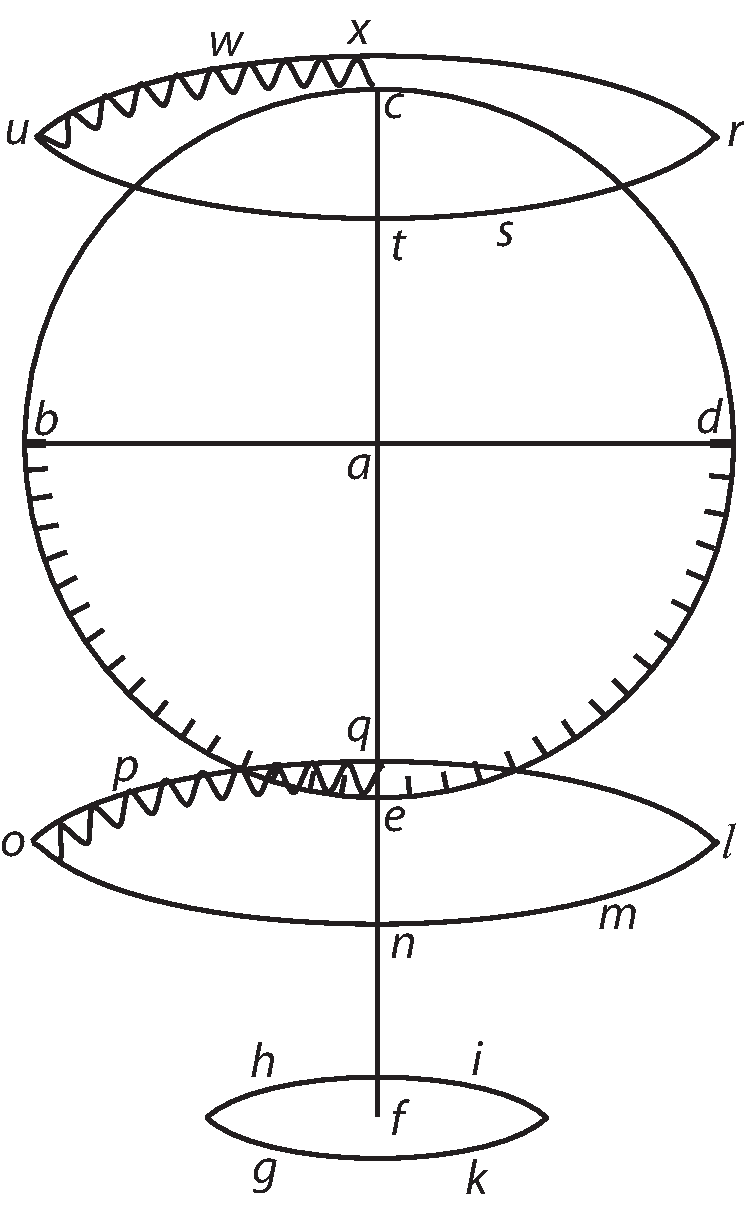
\includegraphics[width=0.7\textwidth]{images/38_201r}
              \vspace{1.0ex}
              \\ \textit{[Fig. 1]} \\
              \end{center}
            ungez\"{a}hnten theils des rades \textit{abcde} wie in der figur zu sehen. Von iedem \edtext{Rad}{\lemma{iedem}\Afootnote{ \textit{ (1) }\ Centro \textit{ (2) }\ Rad \textit{ L}}} ist ein Viertheil gezahnet, iedes mit etwa 13 Z\"{a}hnen damit den L\"{u}cken zwischen den Z\"{a}hnen des rads \textit{abcde} correspondire, nehmlich \textit{opq} im rad \textit{lmnopq} und \textit{uwx} im rad \textit{rstuwx}. Beyde am lincken untern Viertheil iedes rades.\pend \pstart Endtlich soll das rad \textit{abcde} auch eine scheibe Vertreten k\"{o}nnen umb eine chorde \edtext{daran}{\lemma{chorde}\Afootnote{ \textit{ (1) }\ darauf \textit{ (2) }\ daran \textit{ L}}} zu seyen, und also einige dicke und Krinne haben, darin die chorde gehen k\"{o}nne. Dergestalt werden solche R\"{a}der den effect der \textso{Wechselr\"{a}der}\protect\index{Sachverzeichnis}{Wechselr\"{a}der} thun. Und wenn  die stange mit dem gewicht das rad herumb drehet, und gehet aus \textit{k} in \textit{g}. So gehen die Z\"{a}hne \edtext{\textit{opq}  in \textit{ql}}{\lemma{Z\"{a}hne}\Afootnote{ \textit{ (1) }\ \textit{qp} in \textit{ql} \textit{ (2) }\ \textit{opq} in \textit{ql} \textit{ L}}} und die Z\"{a}hne \textit{uwx} in \textit{xr} und die Z\"{a}hne \textit{bed} in \textit{edc}.\pend \pstart Wenn aber die Stange wieder  hinauff gehet aus \textit{g} in \textit{k}. So gehen die Z\"{a}hne aus \textit{xr} wieder in \textit{uwx} und ergreiffen die Z\"{a}hne \textit{bed} in \textit{c} und also obgleich die Stange auff und ab gehet, gehet doch das rad \textit{abcde} auff eine seite herumb.\pend 
            